\documentclass[11pt]{beamer}
\usepackage{graphicx,hyperref}
\usepackage{subfigure}
\usepackage[english]{babel}
\usepackage{times}
\usepackage[T1]{fontenc}
\usepackage{diagbox}
\usepackage[authordate]{biblatex-chicago}
\usepackage{setspace}
\usepackage{chngcntr}
\usepackage[table]{xcolor}
\usepackage{appendixnumberbeamer}
\usepackage{tikz}
\usepackage{csquotes}
\usepackage{longtable}

\usetikzlibrary{arrows,positioning} 
\tikzset{
    %Define standard arrow tip
    >=stealth',
    %Define style for boxes
    punkt/.style={
           rectangle,
           rounded corners,
           draw=black, very thick,
           text width=6.5em,
           minimum height=2em,
           text centered},
    % Define arrow style
    pil/.style={
           ->,
           thick,
           shorten <=2pt,
           shorten >=2pt,}
}
\usepackage{hyperref}
\addbibresource{bib/PoliceResidency.bib}


\usetheme{Madrid}
\definecolor{EmoryBlue}{RGB}{1,33,105}
\usecolortheme[named=EmoryBlue]{structure}



    \title[Estimator Selection]{Estimator Selection Diagnostics in Staggered Differences-in-Differences}
    \author[Eric Dobbie]{Eric Dobbie}
    \institute[Emory]{Emory University\\Department of Political Science} 
    \date{\today}  
    \logo{
\includegraphics[width=1.19cm,height=0.4cm]{slidefigures/School.png}}

\begin{document}
%%%%%%%%%%%%%%%%%%%%%%%%%%%%%%%%%%%%%%%%%%%%%%%%%%%%%%%%%%%%%%%%%%%%%%%%%%%%%%%%%%%%%%
\begin{frame}\titlepage
\end{frame}

\section{Background}

\begin{frame}{Staggered Treatment DiD}
    \begin{itemize}
        \item Common applied DiD settings are complicated, with treatments being applied at different time periods for different geographic units.
        \item These setting are especially common in policy evaluation settings, where policy is not adopted uniformly across different jurisdictions.
        \item Typical applied work used TWFE estimators in these applications
    \end{itemize}
\end{frame}

\section{Staggered Treatments Lead to Bad Comparisons}

\begin{frame}{Goodman-Bacon Bias}
    \begin{itemize}
        \item However, TWFE has a problem. \textcite{goodman2021difference} showed that using TWFE leads to unintuitive comparisons, where the treatment group in a previous period serves as the control group for units treated in the current period.
        \item These comparisons bias the estimate of the ATT when using TWFE models
    \end{itemize}

    The bias term is given by 
    \begin{equation}\label{eq:biastwfe}
        \text{Bias} = \sum_{k \not = U} \sum_{\mathcal{L} > k} \sigma_{k \mathcal{L}} (1 - \mu_{k\mathcal{L}})[ATT_k(POST(\mathcal{L})) - ATT_k(MID(k,\mathcal{L}))]
    \end{equation}
    Which is the change in treatment effect across periods.
\end{frame}

\section{Goodman-Bacon Decomposition}

\begin{frame}{Goodman-Bacon Decomposition}
    \textcite{goodman2021difference} decomposes the TWFE model into all possible 2x2 DiD comparisons.

    \begin{figure}
        \centering
        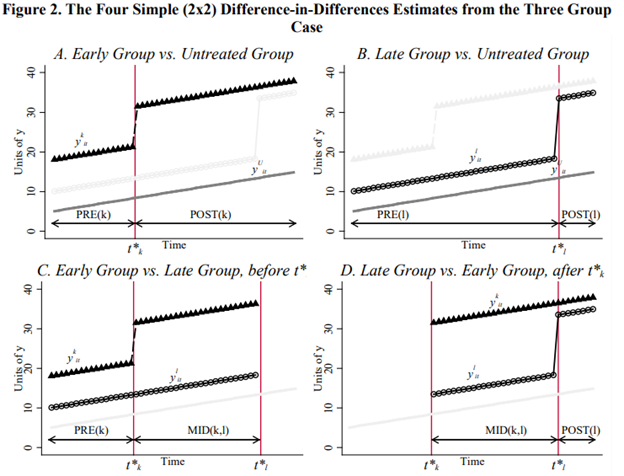
\includegraphics[width=0.7\linewidth]{slidefigures/comparisons.png}
        \label{fig:GB_Decomp}
    \end{figure}
\end{frame}

\begin{frame}{Goodman-Bacon Decomposition}
    There are two (related) problems that arise from this:

    \begin{enumerate}
        \item Some of these comparisons (namely Panel D) are unintuitive, strange comparisons
        \item When we include these strange comparisons, the weights on some of these 2x2 DiD cells can be negative in the aggregation process, leading to biased estimates.
    \end{enumerate}

     Because of these problems, TWFE estimators are generally not advisable in staggered treatment settings
\end{frame}

\section{Reweighting Estimators}

\begin{frame}{The Solution: Restrict Focus to Clean Comparisons}
    There is a class of modern estimators that works by restricting the analysis to clean comparisons of treated groups with not-yet-treated or never-treated control groups.

    \vspace{2.5mm}

    For this paper I will focus on the most widely adopted set of these estimators (\cite{callaway2021difference, sun2021estimating, borusyak2024revisiting,gardner2022two})
\end{frame}

\begin{frame}{Estimator Selection}
    For applied researchers, the following set of questions must be answered:
    \begin{enumerate}
        \item \textbf<2->{Can these estimators give different results for the same underlying data?}
        \item Under what conditions does estimator selection matter?
        \item When estimator selection matters, how do I select which one is correct for my application?
    \end{enumerate}
\end{frame}

\begin{frame}{How do reweighting estimators work?}
    Imagine a setting with $n$ treatment cohorts and $m$ time periods.
    
    \vspace{2.5mm}

    \begin{table}[]
\centering
\begin{tabular}{c|ccccc}
      \diagbox{g}{j}   & 1              & 2              & ...      & m-1              & m              \\ \hline
1        & $\tau_{1,1}$   & $\tau_{1,2}$   & ...      & $\tau_{1,m-1}$   & $\tau_{1,m}$   \\
2        & 0   & $\tau_{2,2}$   & ...      & $\tau_{2,m-1}$   & $\tau_{2,m}$   \\
$\vdots$ & $\vdots$       & $\vdots$       & $\vdots$ & $\vdots$         & $\vdots$       \\
n-1      & 0 & 0 & ...      & $\tau_{n-1,m-1}$ & $\tau_{n-1,m}$ \\
n        & 0  & 0   & ...      & $\tau_{n,m-1}$   & $\tau_{n,m}$  
\end{tabular}
\end{table}

    With treatment in period $k_i$, let $i \in [1,n]$ index treatment cohorts and $j \in [1,m]$ index time period, where $j \in [1,k_i)$ represent pre-treatment periods for each cohort and $j \in [k_i,m]$ represent treated periods. Each $\tau_{i,j}$ represents the cohort by period ATT, 
    \begin{equation}
        \tau_{i,j} = E[Y_{it}(1) - Y_{it}(0) | j \geq k_i ]
    \end{equation}

\end{frame}

\begin{frame}{Aggregating to the ATT}    
    \textcite{callaway2021difference} propose that researchers should use these as a target estimand and directly report these $\tau_{i,j}$ values. 

    \vspace{2.5mm}
    
    However, in settings where $i$ and/or $j$ are large, the number of $\tau_{i,j}$ values will be too large to take away substantive conclusions. 
    
\vspace{2.5mm}
    
    Therefore, many applied researchers look to aggregate these cohort by period effects into a more familiar aggregate ATT.
\end{frame}

\begin{frame}{Reasonable Aggregation Schemes}
    In order to aggregate these $\tau_{i,j}$ estimates, one can imagine several possible approaches:

    \begin{itemize}
        \item Aggregating over cohorts to generate event study or calendar estimates with period specific effects
        \item Aggregating over periods to generate cohort specific effects
        \item Aggregating over both periods and cohorts to generate a single ATT
    \end{itemize}
\end{frame}

\begin{frame}{Event Study Aggregation}
    For event study aggregation, the target is to reduce from $\tau_{i,j}$ to period specific effects, $\theta_{es}(e)$, where $e$ represents the number of periods since treatment for each cohort $i$. Formally, $e = j - k_i$. The event study estimate is given by:
    \begin{equation}
        \theta_{es}(e) = \sum_i w_{i,e} \tau_{i,e}
    \end{equation}

    Note that $e$ is cohort specific, such that $e = 1$ can be in different time periods $j$ for each cohort. 
\end{frame}

\begin{frame}{Event Study Aggregation}
    Consider an example with 5 time periods and 4 treatment cohorts, treated in periods 2 to 5 sequentially, such that cohort 1 is treated in period 2, cohort 2 is treated in period 3, and so on.
    \begin{table}[]
\centering
\begin{tabular}{c|ccccc}
      \diagbox{i}{j}   & 1              & 2              & 5      & 4             & 5              \\ \hline
1        & $\tau_{1,1}$   & $\tau_{1,2}$   & $\tau_{1,3}$    & $\tau_{1,4}$   & $\tau_{1,5}$   \\
2        & $\tau_{2,1}$   & $\tau_{2,2}$   & $\tau_{2,3}$      & $\tau_{2,4}$   & $\tau_{2,5}$   \\
3      & $\tau_{3,1}$ & $\tau_{3,2}$ &  $\tau_{3,3}$     & $\tau_{3,4}$ & $\tau_{3,5}$ \\
4        & $\tau_{4,1}$   & $\tau_{4,2}$   & $\tau_{4,3}$     & $\tau_{4,4}$   & $\tau_{4,5}$  
\end{tabular}
\end{table}
\end{frame}

\begin{frame}{Event Study Aggregation}
    To estimate $\theta_{es}(1)$, the blue cells are added together using a weighted average, $\theta_{es}(2)$ is a weighted average of green cells, $\theta_{es}(3)$ is a weighted average of the purple cells, and $\theta_{es}(4) = \tau_{1,5}$, the orange cell, by construction:

    \begin{table}[]
\centering
\begin{tabular}{c|ccccc}
      \diagbox{g}{j}   & 1              & 2              & 3      & 4             & 5              \\ \hline
1        & 0   &\cellcolor{blue!30} $\tau_{1,2}$   & \cellcolor{green!30}$\tau_{1,3}$    & \cellcolor{purple!30}$\tau_{1,4}$   &\cellcolor{orange!30} $\tau_{1,5}$   \\
2        & 0   & 0  & \cellcolor{blue!30}$\tau_{2,3}$      & \cellcolor{green!30}$\tau_{2,4}$   & \cellcolor{purple!30}$\tau_{2,5}$   \\
3      & 0 & 0 &  0     & \cellcolor{blue!30}$\tau_{3,4}$ & \cellcolor{green!30}$\tau_{3,5}$ \\
4        & 0  & 0   & 0     & 0   & \cellcolor{blue!30}$\tau_{4,5}$  
\end{tabular}
\end{table}
\end{frame}

\begin{frame}{Event Study Aggregation}
    The weights, $w_{i,e}$, depend on the estimator. \textcite{sun2021estimating} weigh by cohort-period shares such that, in the example:
    \begin{equation}
        \theta_{es}(e) = \frac{n_{i=1, e}}{n_{e}} \tau_{1,e} + \frac{n_{i=2, e}}{n_{e}} \tau_{2,e}+\frac{n_{i=3, e}}{n_{e}} \tau_{3,e}+\frac{n_{i=4, e}}{n_{e}} \tau_{4,e}
    \end{equation}

    Where $\frac{n_{i,e}}{n_e}$ is the share of that event period sample size from that treatment cohort. For $e = 2$, for example:

    \begin{align*}
                \theta_{es}(2) &= \frac{n_{i=1, 2}}{n_{2}} \tau_{1,2} + \frac{n_{i=2, 2}}{n_{2}} \tau_{2,2}+\frac{n_{i=3, e}}{n_{2}} \tau_{3,e}+\frac{0}{n_{2}} \tau_{4,2} \\
                & = \frac{n_{i=1, 2}}{n_{2}} \tau_{1,2} + \frac{n_{i=2, 2}}{n_{2}} \tau_{2,2}+\frac{n_{i=3, e}}{n_{2}} \tau_{3,e}
    \end{align*}
\end{frame}

\begin{frame}{Calendar Effects}
    Another approach uses a calendar specific aggregation. Instead of normalizing to event time, one might be interested in the treatment effect at different points in time, so we aggregate over treatment cohorts within period $j$, for each cohort $i$ such that $j > k_i$.
    \begin{equation}
        \theta_c(j) = \sum_{i;j > k_i} w_{i,j} \tau_{i,j}
    \end{equation}
\end{frame}

\begin{frame}{Calendar Effects}
    Carrying forward the previous example,  $\theta_{c}(1) = \tau_{1,2}$, the blue cell, $\theta_{c}(2)$ is a weighted average of green cells, $\theta_{c}(3)$ is a weighted average of the purple cells, and $\theta_{c}(4)$ is a weighted average of the orange the orange cells.

    \input{tables/calendar/ex_cal}
\end{frame}

\begin{frame}{Cohort Specific Effects}
    One could similarly imagine being interested in estimating the effects of a policy on each treatment cohort. For this, one would want to aggregate across time periods. 

    \begin{equation}
        \alpha_i = \sum_{j > k_i} w_{i,j} \tau_{i,j}
    \end{equation}
\end{frame}

\begin{frame}{Cohort Specific Effects}
    Returning to the example, to find cohort effects we aggregate over time within cohorts, so $\alpha_1$ is a weighted average of the blue cells, $\alpha_2$ is a weighted average of the green cells, $\alpha_3$ is a weighted average of the purple cells, and $\alpha_4 = \tau_{4,5}$, the orange cell.
    \begin{table}[]
\centering
\begin{tabular}{c|ccccc}
      \diagbox{i}{j}   & 1              & 2              & 3      & 4             & 5              \\ \hline
1        & $\tau_{1,1}$   &\cellcolor{blue!30} $\tau_{1,2}$   & \cellcolor{blue!30}$\tau_{1,3}$    & \cellcolor{blue!30}$\tau_{1,4}$   &\cellcolor{blue!30} $\tau_{1,5}$   \\
2        & $\tau_{2,1}$   & $\tau_{2,2}$   & \cellcolor{green!30}$\tau_{2,3}$      & \cellcolor{green!30}$\tau_{2,4}$   & \cellcolor{green!30}$\tau_{2,5}$   \\
3      & $\tau_{3,1}$ & $\tau_{3,2}$ &  $\tau_{3,3}$     & \cellcolor{purple!30}$\tau_{3,4}$ & \cellcolor{purple!30}$\tau_{3,5}$ \\
4        & $\tau_{4,1}$   & $\tau_{4,2}$   & $\tau_{4,3}$     & $\tau_{4,4}$   & \cellcolor{orange!30}$\tau_{4,5}$  
\end{tabular}
\end{table}
\end{frame}

\begin{frame}{Single ATT Aggregation}
    The ATT for each of these reweighting estimators follows this general form:

    \begin{equation}\label{eq:delta}
        \delta = \sum_{i,j>k} w_{ij} * \tau_{ij}
    \end{equation}

    Where $w_{i,j} > 0$ and $\sum_{i,j} w_{i,j} = 1$
\end{frame}

\begin{frame}{Single ATT Aggregation}
    To obtain a single ATT, all treated cells are combined using a weighted average to estimate $\delta$

    \input{tables/att/att}
\end{frame}

\begin{frame}{Aside: Are the $\tau_{i,j}$ values equivalent across estimators?}
Short answer: Sometimes

\vspace{2.5mm}

\textcite{callaway2021difference} and \textcite{sun2021estimating} follow the same decomposition procedure, so they are implicitly dealing with the same $\tau$ matrix with different weighting processes.

\vspace{2.5mm}

We need a parallel trends assumption for \textcite{gardner2022two} and \textcite{borusyak2024revisiting} to produce the same $\tau$ matrix in expectation.
    
\end{frame}

\begin{frame}{Estimator Equivalence Under Parallel Trends}
    \textcite{gardner2022two} uses a two-stage regression approach that can be reduced to the $\tau_{i,j}$ estimation and weighting approach. The first stage residualizes the outcome variable using untreated observation unit and period fixed effects:
    \begin{equation}
        \tilde{Y}_{i,j} = Y_{i,j} - \hat{\alpha}_i - \hat{\gamma}_j
    \end{equation}

    The second stage regresses $\tilde{Y}_{i,j}$ on the treatment for all observations, giving the following coefficient:

    \begin{equation}
        \hat{\delta}_G = \frac{\sum_{i,j} D_{i,j} \tilde{Y}_{i,j}}{\sum_{i,j}D_{i,j}}
    \end{equation}

    Note that $\tilde{Y}_{i,j}$, therefore, gives the cohort-time specific ATT estimates (or, $\tau_{i,j}$) for the Gardner estimator).
\end{frame}

\begin{frame}{Estimator Equivalence Under Parallel Trends}
    \textcite{borusyak2024revisiting} uses an imputation approach, using untreated observations to estimate the counterfactual potential outcomes for each treated unit. They report a single ATE
    \begin{equation}
        \hat{\delta}_{BJS} = \frac{\sum_{i,j} D_{i,j} (Y_{i,j} - \tilde{Y}_{i,j} (0))}{\sum_{i,j}D_{i,j}}
    \end{equation}

    Therefore, the $\tau_{i,j}$ values for \textcite{borusyak2024revisiting} are given by the total effect divided by the share of the sample that comes from that cohort-period cell.

    \begin{equation}
        \tau_{i,j} = \frac{\hat{\delta}_{BJS}}{N_{i,j}}
    \end{equation}

    Under parallel trends, the counterfactual estimation procedure in \textcite{borusyak2024revisiting} is equivalent to the \textcite{gardner2022two} process. This means that, not only are the $\tau_{i,j}$ matrices equivalent, the estimators actually produce identical results when parallel trends hold.
\end{frame}

\begin{frame}{Asymptotic $\tau$ Matrix Equivalence}
    Note that all of these estimators use consistent procedures to estimate these $\tau$ values. This means that, as $N \rightarrow \infty$, the estimators $\hat{\tau}_{i,j} \rightarrow_p \tau_{i,j}$.
    \vspace{2.5mm}

    Therefore, asymptotically, each estimator differs only in the weighting procedure. This makes \textcite{gardner2022two} and \textcite{borusyak2024revisiting} asymptotically equivalent estimators.
\end{frame}

\begin{frame}{Can Estimators Vary?}
    Can estimates of $\delta$, the ATT, vary across estimators?

    \textbf{Yes.}

    \vspace{2.5mm}
    We can return to our general form to see why. When the $\tau$ matrix is fixed across estimators then each unique estimator simply provides a weighting vector $w$ to solve equation \ref{eq:delta}.

    \vspace{2.5mm}

    Different weighting procedures will produce different estimates under certain conditions. It is possible for the weighted averages to produce equivalent estimates by chance, but under certain conditions these estimators can produce different estimates as they have different weights.
\end{frame}

\begin{frame}{When will we observe estimator differences?}
    On to the second key question: Under what conditions does estimator selection matter?

    \vspace{2.5mm}

    We have shown that the $\tau_{i,j}$ matrix is asymptotically equivalent across estimators, so the driving difference will be derived from the weights. When will different weights matter?
\end{frame}

\begin{frame}{Differences Across Estimators}
    We can express the difference between any two reweighting estimators, with estimates $\hat{\tau}$ and $\hat{\tau}^\prime$, with weighting vector $w$ and $w^\prime$:
    \begin{equation}
        \hat{\tau} - \hat{\tau}^\prime = w\tau - w^\prime \tau = (w - w^\prime) \tau
    \end{equation}

    Observation: The magnitude of disagreement between any two fixed estimators is increasing in the variance of the $\tau_{i,j}$ values.
\end{frame}

\section{A Diagnostic Test for Estimator Selection}

\begin{frame}{$Var(\tau_{i,j})$ as a diagnostic tool}
    Note that, the lower the variance in $\tau_{i,j}$ values, the less our weighting choice matters. In the case with no heterogeneous effects, such that Var$(\tau_{i,j})=0$, the difference in the weighting vectors is completely inconsequential, such that the difference between the estimators is, necessarily, zero. 

    \vspace{2.5mm}

    Based on this intuition, I propose using the variance in $\hat{\tau_{i,t}}$ as a diagnostic tool for sensitivity to estimator selection.
\end{frame}

\section{Simulation}

\begin{frame}{Simulation Study}
    I will now show that the $\tau_{i,j}$ variance predicts estimator variance using a simulation study. I operationalize $\tau_{i,j}$ as the ATT(g,t) estimates from \textcite{callaway2021difference}.
    \vspace{2.5mm}

    For this simulation, I draw 1000 datasets using the following data generating process:

    \begin{itemize}
        \item $N = 300$, with 4 equal cohorts with $N = 75$.
        \item 12 periods
        \item 3 treated cohorts with treatment in $k = \{3,6,9\}$
        \item $Y \sim N(0,2) + \tau_{i,j}$
        \item $\tau_{i,k} \sim N(3,5)$
        \item in period $k+m$, $\tau_{i, j = k+m} = \tau_{i,k} + g_{i} * m$
        \item $g_i \sim N(0,0.5)$
        \item Variation in pretreatment trends to simulate violation of parallel trends, $t \sim N(0,0.4)$
    \end{itemize}
\end{frame}

\begin{frame}{Simulation Results}
    \begin{figure}
        \centering
        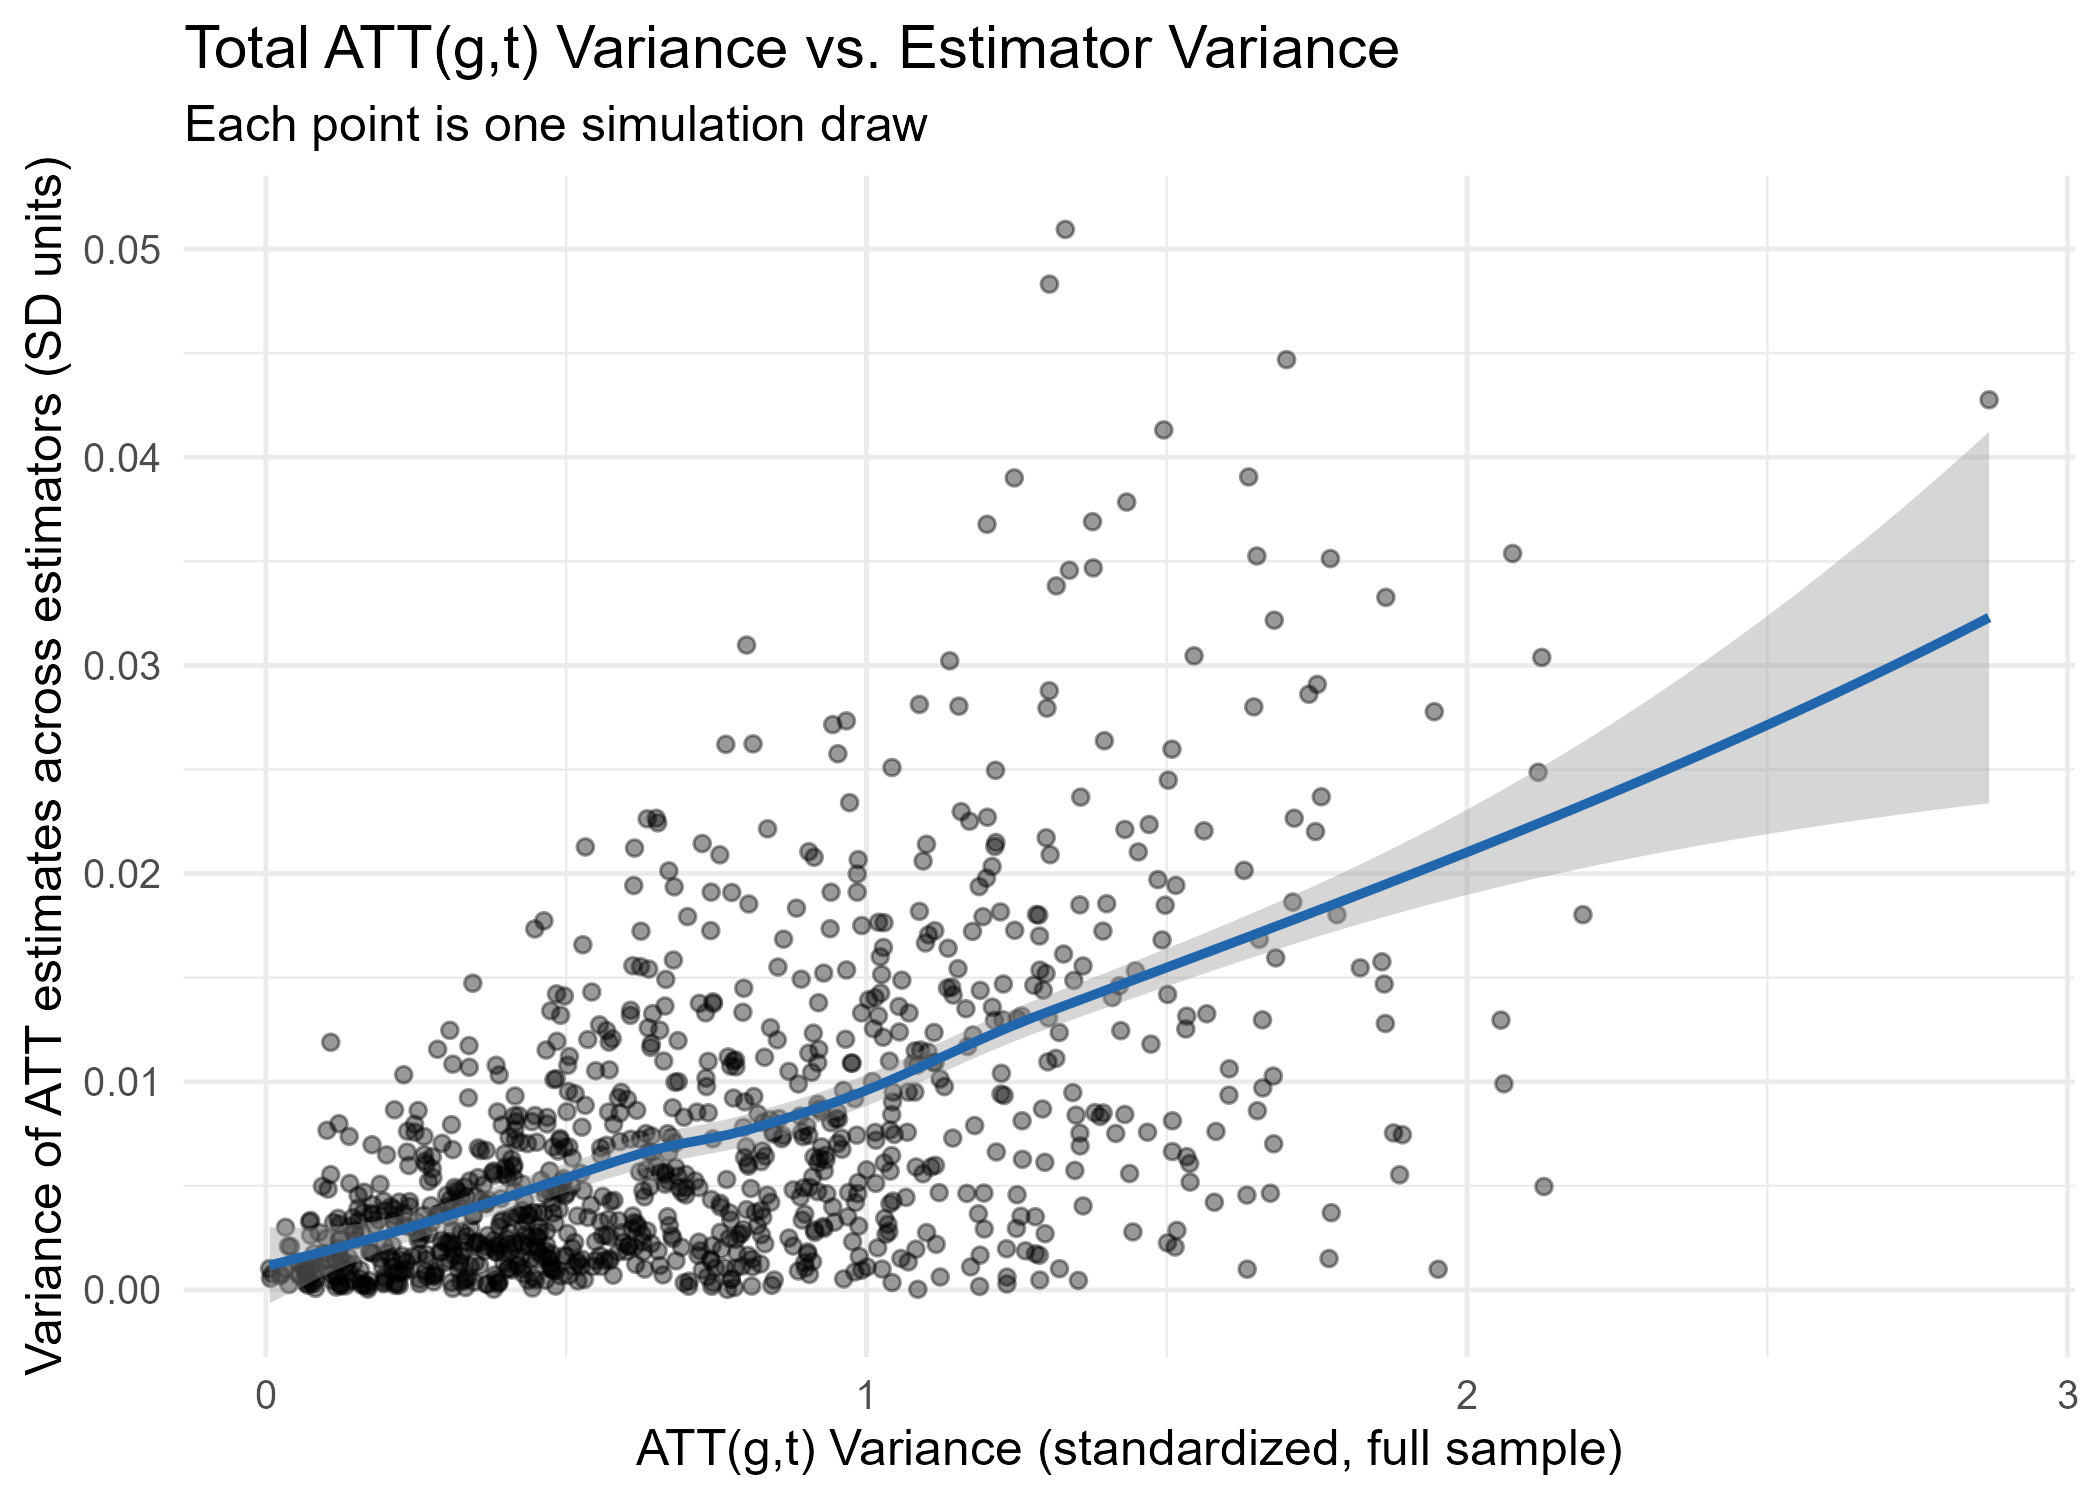
\includegraphics[width=0.75\linewidth]{figures/simulation/diag_attgt_vs_estvar.png}
        \caption{Estimator Variance and ATT(g,t) variance}
        \label{fig:sim1}
    \end{figure}
\end{frame}

\begin{frame}{Simulation Results}
\begin{figure}
    \centering
    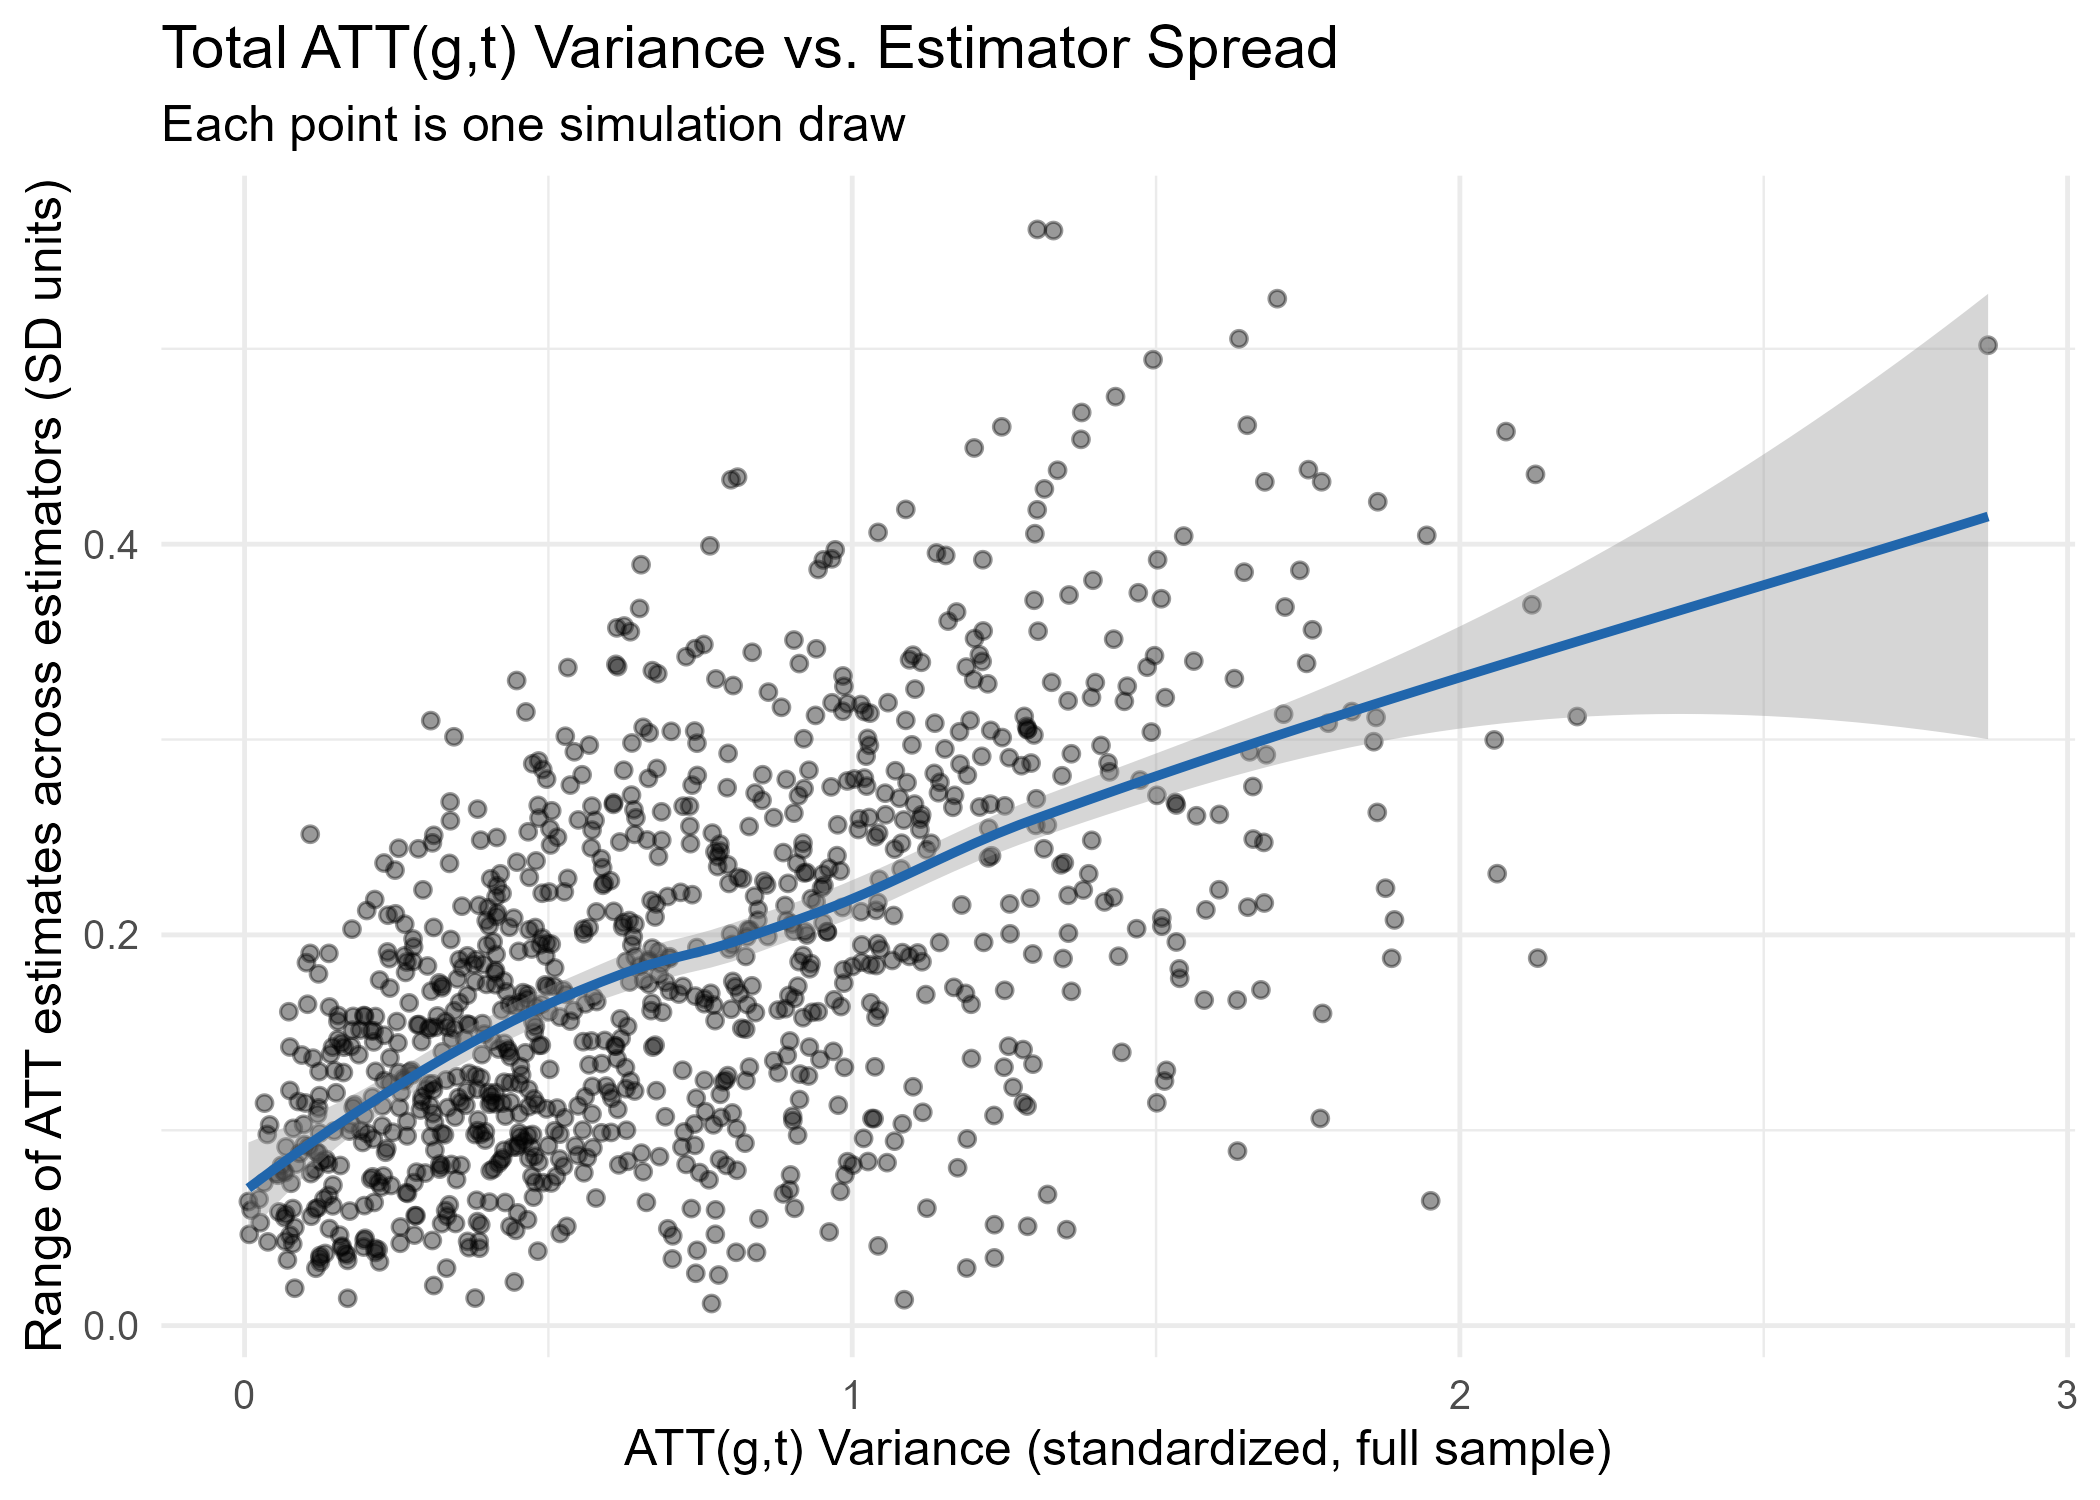
\includegraphics[width=0.75\linewidth]{figures/simulation/diag_gb_vs_spread.png}
    \caption{Estimator Range and ATT(g,t) Variance}
    \label{fig:placeholder}
\end{figure}
    
\end{frame}

\begin{frame}{Simulation Results}
    \begin{figure}
        \centering
        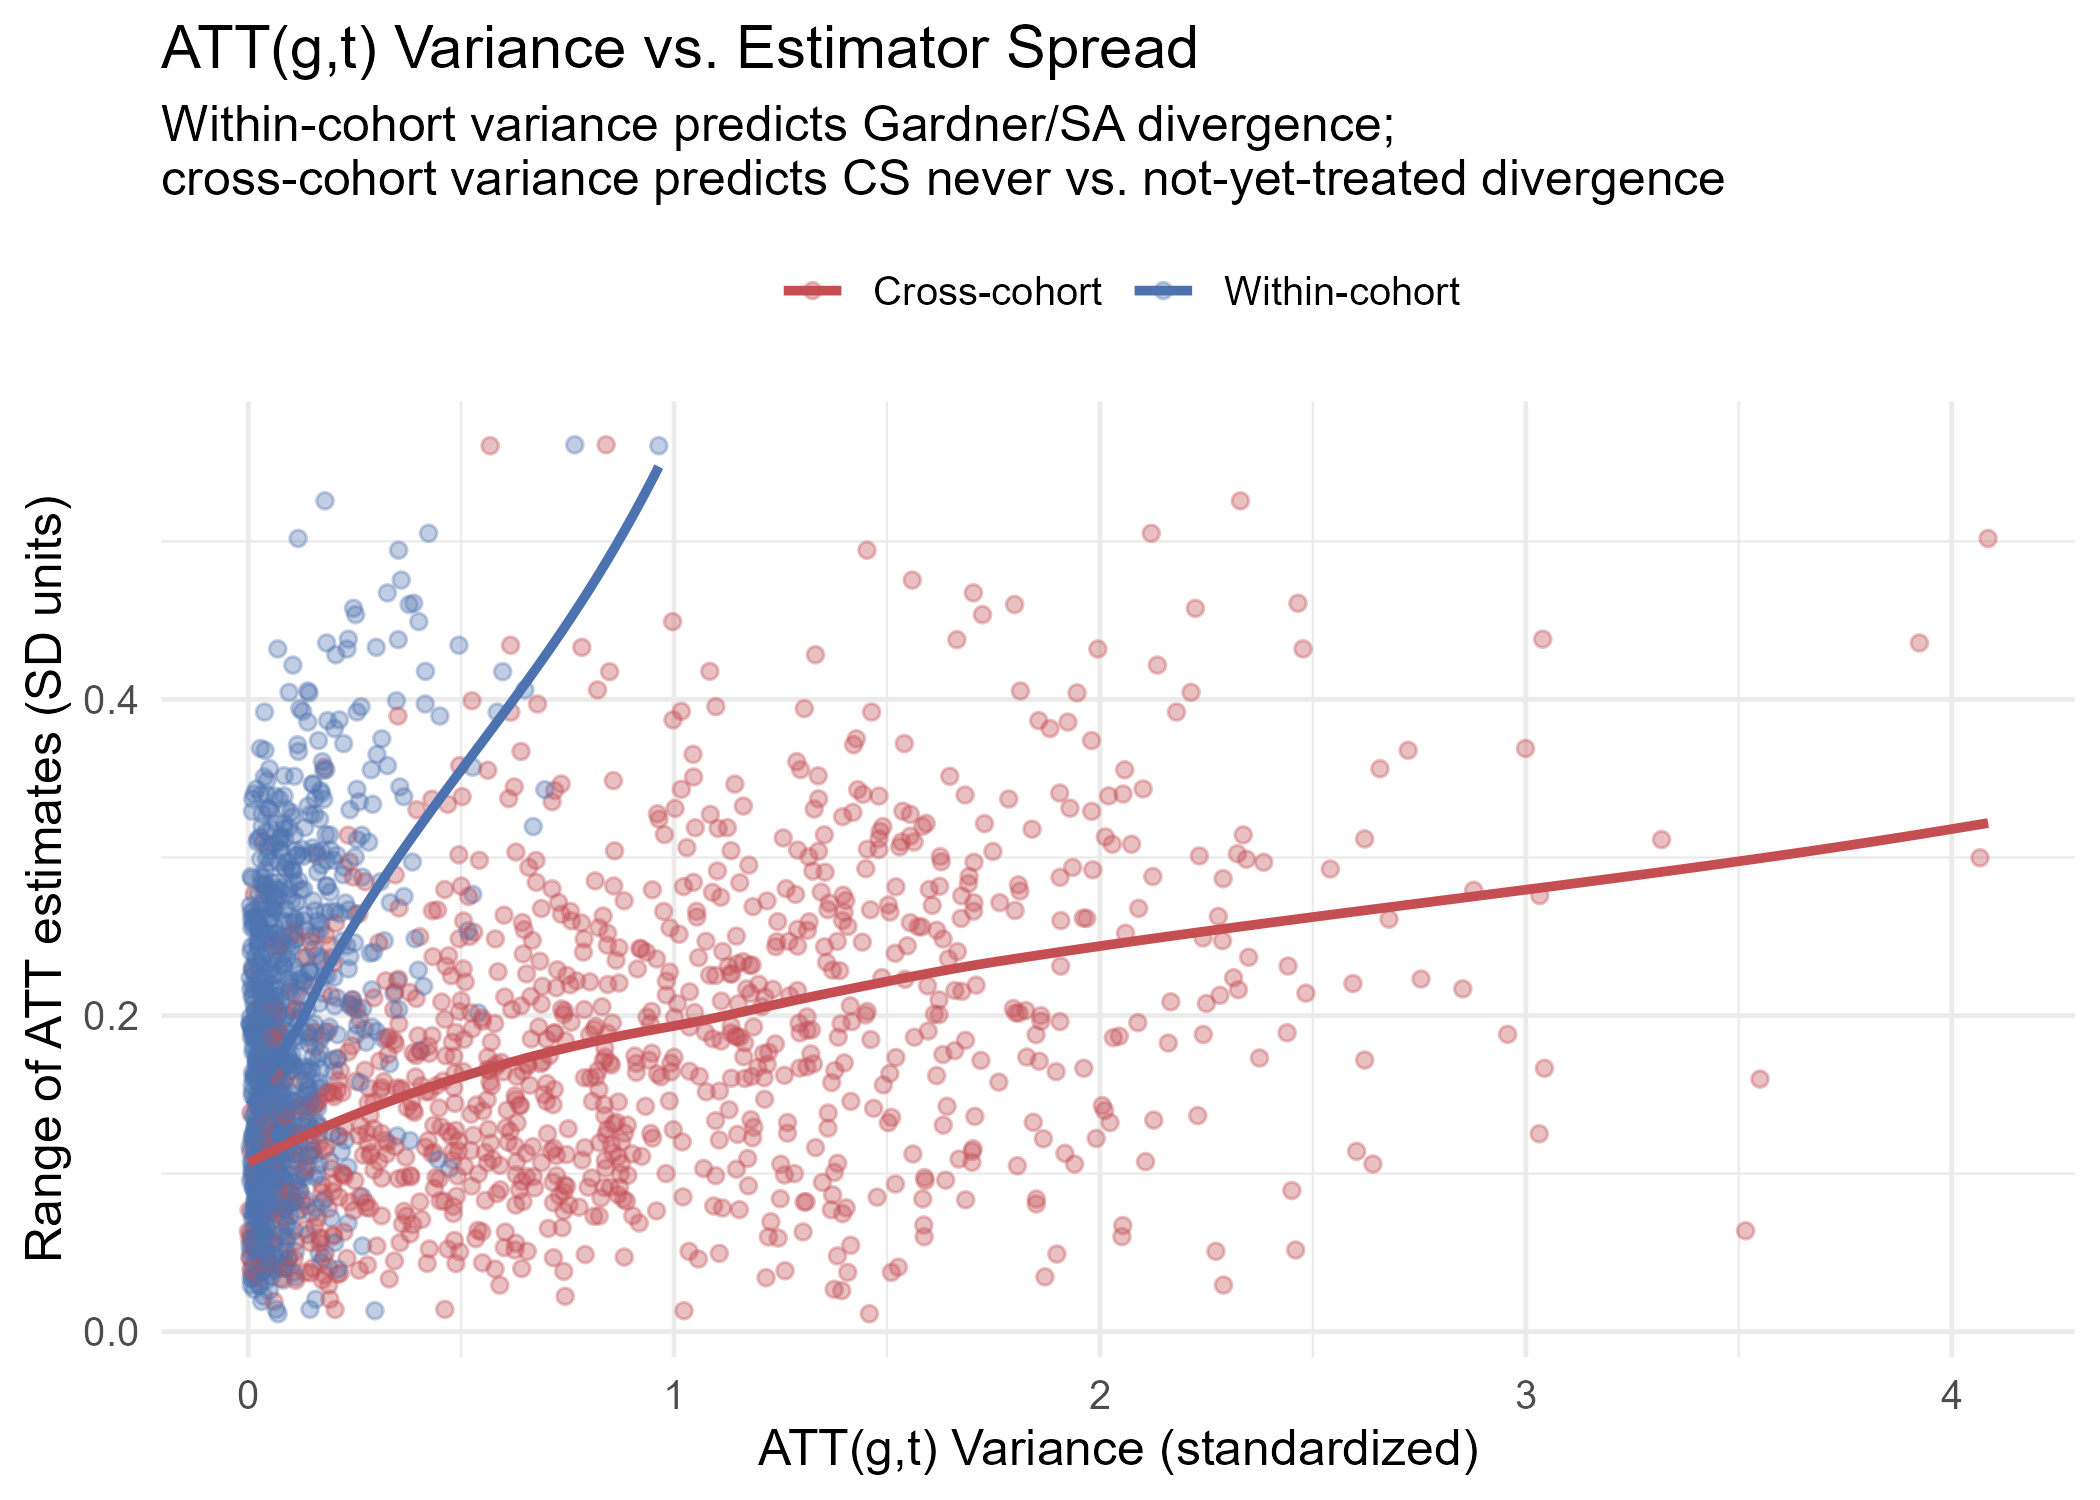
\includegraphics[width=0.75\linewidth]{figures/simulation/diag_gb_components.png}
        \caption{Within and Across Cohort Variance and Estimator Range}
        \label{fig:placeholder}
    \end{figure}
\end{frame}

\begin{frame}{What drives estimator range?}
    \begin{enumerate}
        \item There are no differences between \textcite{gardner2022two} and \textcite{borusyak2024revisiting}.
        \item The largest differences are driven by \textcite{sun2021estimating} being far away from the rest of the estimators. This does not necessarily mean that \textcite{sun2021estimating} is underperforming uniformly, the opposite is also be true depending on the data generating process
    \end{enumerate}
\end{frame}

\section{Application}

\end{document}